\documentclass[10pt,letterpaper]{article}
\usepackage[utf8]{inputenc}
\usepackage[english]{babel}
\usepackage{amsmath}
\usepackage{amsfonts}
\usepackage{amssymb}
\usepackage{graphicx}

\author{Benjamin Peter}
\title{Analysis of Kellis-Birrer-Landis}

\newcommand{\CS}{\mathcal{S}}
\newcommand{\BP}{\mathbb{P}}
\newcommand{\BE}{\mathbb{E}}
\newcommand{\BI}{\mathbb{I}}
\newcommand{\BR}{\mathbb{R}}
\newcommand{\CT}{\mathcal{T}}
\newcommand{\bb}[1]{\mathbf{#1}}



\begin{document}
\maketitle

\section{Accelerated evolution}
The authors constructed a phylogeny as follows: Let $K$ denote the outgroup species, $Y$ and $Z$ the two S. c. paralogs. Let $D(K,Y|G)$, $D(K,Z|G)$ and $D(Y,Z|G)$ be the number of nucleotide substitutions observed between the pairs of gene sequences. Then, the transformed statistics
\begin{equation*}
\begin{split}
S(Z |G, K,Y) = \frac{1}{2}(D(K,Z|G)+D(Y,Z|G)-D(K,Y|G))\\
S(Y |G, K,Z) = \frac{1}{2}(D(K,Y|G)+D(Y,Z|G)-D(K,Z|G))\\
S(K |G, Y,Z) = \frac{1}{2}(D(K,Z|G)+D(K,Z|G)-D(Y,Z|G))
\end{split}
\end{equation*}
give the branch-specific mutations, i.e. the number of sites where two of the genome agree, but not the third. I'll omit the dependencies on the other two genotypes and just write $S(Z)$ for brevity.

Then, the test of accelerated evolution is equivalent to testing the hypothesis that $S(K)=\frac{(S(Y)+S(Z)}{2}$, with alternative hypothesis $S(K)<\frac{(Z)+S(Y)}{2}$. The idea of the approach is that substitutions accumulate due to a molecular clock at a rate that is constant with time from the common ancestor of the three species. They reject the null hypothesis when
\begin{equation*}
\frac{S(Z)+S(Y)}{2 S(K)} > 1.5
\end{equation*}
or something similar. I could not reproduce that result from their data, however the set of 76 genes is given and can be found intersecting the tables included \texttt{S9\_Trees/Duplicated\_Pairs.xls} and         
\texttt{S9\_Trees/Nucleotide\_Divergence.xls} files from the supplement. The $S$ values can be calculated from the alignments provided in the supplement to the paper, where I ignored loci that showed gaps in any of the three sequences.

The first figure shows that the data for these 76 gene more or less supports the claim in the paper that one gene shows similar divergence $S_z$ than the outgroup gene $S_K$, whereas the other copy looks different (note that I ordered the gene copies such that $S_Y < S_Z$.
\begin{figure}[h!]
  \caption{Seems reaonable..}
  \centering
    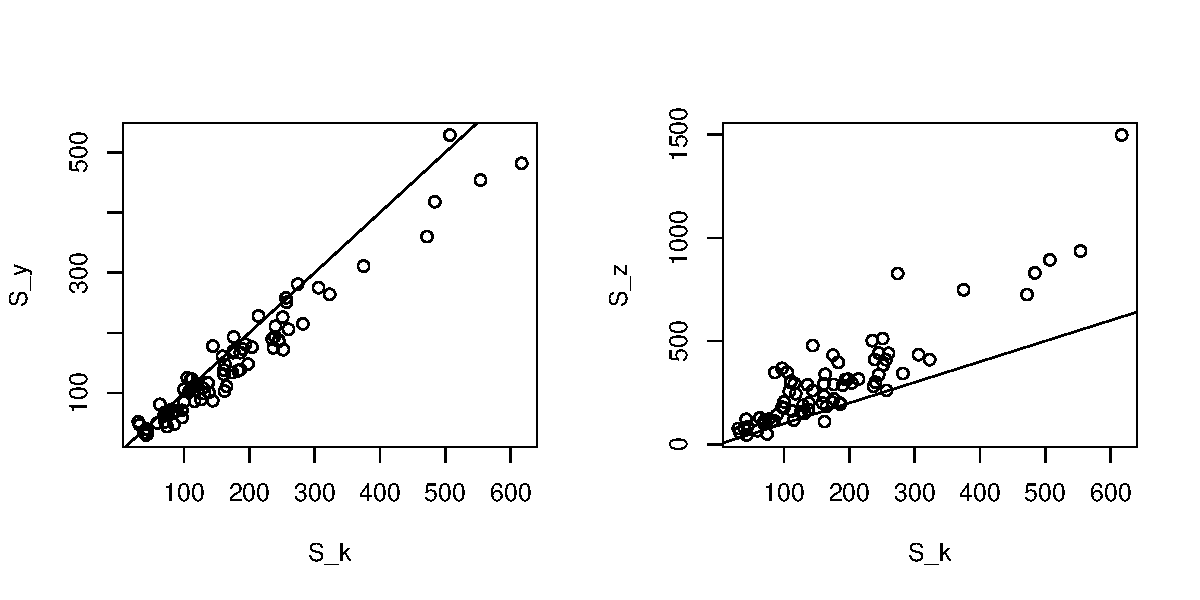
\includegraphics[width=1.2\textwidth]{kellis1.pdf}
\end{figure}

For the test Lior asked about, we look at all pairs of genes that are identified as having an accelerated rate, and figure out if there are one or two rates of acceleration. We can formulate that in the following hypotheses
\begin{enumerate}
\item $\bb{H_0}$: $S_k < S_y, S_k < S_z$ (two different rates of accelerated evolution)
\item $\bb{H_1}$: $S_k = S_y, S_k < S_z$ (one rate of accelerated evolution)
\end{enumerate}
Assuming that mutations are independent, $S_k$, $S_y$ and $S_z$ are distributed multinomially with likelihood
\begin{align*}
L = \log\left[\left(\sum S_i)\right)!\right] - \sum \log{S_i} + \sum S_i * p_i
\end{align*}
where all sums are over $(k, y, z)$.
For $\bb{H_0}$, we find $p_k$, $p_y = p_k + p_y$ and $p_z = p_k + i_z$ subject to the constraints 
$p_z + p_k + p_y =0, i_z \geq 0 i_y \geq 0$.
For $\bb{H_1}$, we use the same likelihood, but with constraint $i_y=0$. For a classical likelihood-ratio test, we would want to have the hypotheses switched, but looking at the data reveals that for 62 of the 76 samples, the maximum likelihood estimate of $i_y$ is zero. So for these 62 samples, we would prefer $\bb{H_1}$ under pretty much any framework. Indeed, using BIC, we find that $\bb{H_0}$ is preferred over $\bb{H_1}$ for all samples. Similarly, looking at the statistic $D = 2* L(\bb{H_0} - L(\bb{H_1})$ shows that only four of the values have a D greater than 2. As we would expect $D$ to be $\chi^2_1$ distributed, it is clear that the vast majority of genes are consistent with the claimed ``only one of the genes shows accelerated evolution''. It probably would be possible to wrangle that into a statement about $p$-values (and I fear if somebody did that, Lior might go bankrupt), but it does not seem worth the effort.

As a biologist, that is not really surprising; these are likely loss-of-function mutations and have probably little to do with any functionality.



\begin{figure}[h!]
  \caption{Tests}
  \centering
    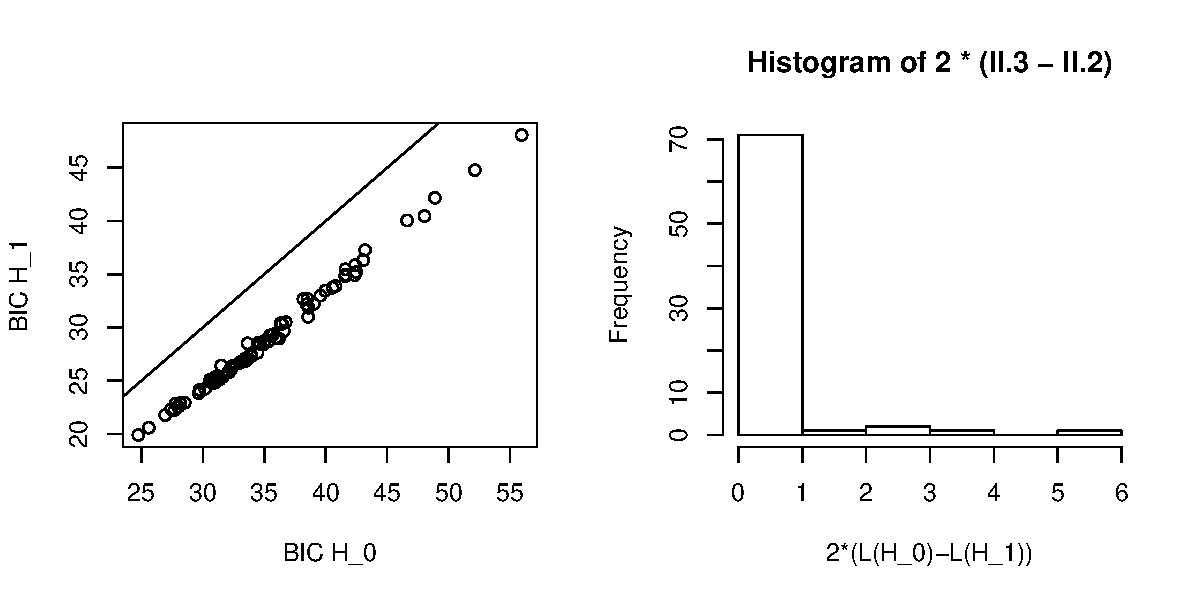
\includegraphics[width=1.2\textwidth]{kellis2.pdf}
\end{figure}

\end{document}
